%-------------------------
% Resume in LaTeX -- Wenhao Wu
%------------------------
\documentclass[a4paper,11pt]{article}
\usepackage[margin=1.35cm]{geometry}
\usepackage{fontspec}
\usepackage{xeCJK}
\setCJKmainfont{Droid Sans Fallback}
\usepackage{xcolor}
\usepackage{graphicx}
\usepackage{tabularx}
\usepackage{enumitem}
\usepackage[hidelinks]{hyperref}
\usepackage{titlesec}
\usepackage{array}
\usepackage{amssymb}
\pagestyle{empty}
\setlength{\parindent}{0pt}
\setlength{\parskip}{0pt}
\setlist[itemize]{leftmargin=1.4em,itemsep=1pt,topsep=2pt,parsep=0pt}
\titleformat{\section}{\large\bfseries\scshape}{}{0em}{}[\titlerule]
\titlespacing*{\section}{0pt}{8pt}{4pt}
\newcommand{\entry}[2]{\textbf{#1}\hfill\textit{#2}\\}
\newcommand{\paper}[3]{\item \textbf{#1}\\{\small #2}\\{\small #3}\vspace{3pt}}

\begin{document}

% Photo: replace the file path below if the portrait is moved.
\begin{minipage}[c]{2.25cm}
  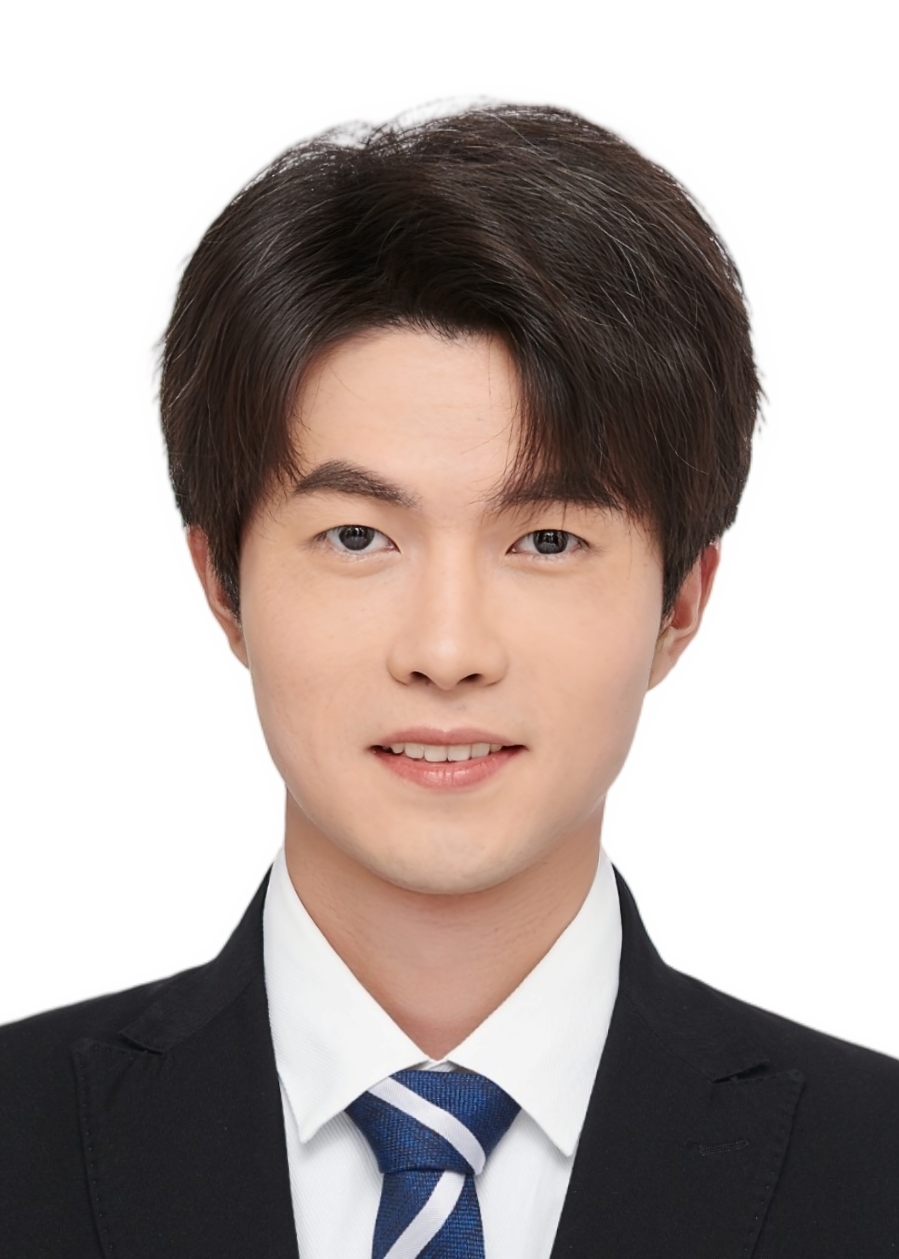
\includegraphics[width=2.25cm,height=2.55cm,keepaspectratio]{photo.jpg}
\end{minipage}\hspace{0.35cm}
\begin{minipage}[c]{\dimexpr\linewidth-2.6cm\relax}
  {\LARGE\bfseries Wenhao Wu (吴文浩)}\\[3pt]
  Master's Student \enspace|\enspace Nanjing University\\
  (+86) 18005527326 \enspace
  Email: \href{mailto:wenhaowu@smail.nju.edu.cn}{wenhaowu@smail.nju.edu.cn}\\
  Homepage: \href{https://wuwenhao09.github.io/}{wuwenhao09.github.io} \enspace
  \href{https://scholar.google.com/citations?user=qiQb1BMAAAAJ}{Google Scholar}
\end{minipage}

\section{Research Interests}
Large Language Model Agents, Retrieval-Augmented Generation, Meta Reinforcement Learning, and Vision-Language-Action.

\section{Education}
\entry{Nanjing University, School of Management and Engineering}{09/2024--Present}
M.Eng. in Control Engineering; supervised by Prof. Zhi Wang.\\[2pt]
\entry{Nanjing University, School of Management and Engineering}{09/2020--06/2024}
B.Eng. in Automation.

\section{Research Experience}
\begin{itemize}[leftmargin=1.4em,label=\textbullet,itemsep=6pt,topsep=2pt]\paper{MemFuse: Multi-Source Memory Fusion from Fragmented Observations}{\href{https://arxiv.org/abs/2608.18704}{arXiv preprint, 2026}; co-author}{Chao Li, Yuanfa Li, \textbf{Wenhao Wu}, Xule Liu, Zhi Wang, Kun Shao.}
Introduces MemFuseBench for multi-source memory fusion and a dual-layer causal fusion graph that preserves source provenance while organizing fragmented observations into retrievable memories.\par

\paper{From Conflict to Consensus: Boosting Medical Reasoning via Multi-Round Agentic RAG}{\href{https://openreview.net/forum?id=S7lpdz7NAW}{ICML 2026}; first author}{\textbf{Wenhao Wu}, Zhentao Tang, Yafu Li, Shixiong Kai, Mingxuan Yuan, Zhenhong Sun, Chunlin Chen, Zhi Wang.}
Proposed conflict-guided multi-round retrieval for medical reasoning, using disagreement among sampled responses to generate precise queries and sequence-level entropy or a lightweight BERT verifier to rerank historical reasoning trajectories.\par

\paper{Look Before You Leap: Distilling Tree Search into Action Evaluation for Frozen VLA Models}{\href{https://arxiv.org/abs/2607.03751}{arXiv preprint, 2026}; co-author}{Xinyi Xie, Zican Hu, Zhanyu Liu, Yicheng Dong, \textbf{Wenhao Wu}, Haoran Li, Chunlin Chen, Zhi Wang*, Pichao Wang.}
Proposed SVA (Search, Value, and Act), which keeps the VLA backbone frozen and distills Monte-Carlo tree search into a lightweight Q-value evaluator that selects the best of N candidate actions at deployment without simulator access.\par

\paper{Mixture-of-Experts Meets In-Context Reinforcement Learning}{\href{https://proceedings.neurips.cc/paper_files/paper/2025/hash/233cbc888ef01917d8d895e471e80a01-Abstract-Conference.html}{NeurIPS 2025}; first author}{\textbf{Wenhao Wu}, Fuhong Liu, Haoru Li, Zican Hu, Daoyi Dong, Chunlin Chen, Zhi Wang.}
Proposed T2MIR, a dual-MoE framework with Token-wise and Task-wise experts for multi-modal trajectory processing and multi-task in-context RL.\par

\paper{Text-to-Decision Agent: Offline Meta-Reinforcement Learning from Natural Language Supervision}{\href{https://proceedings.neurips.cc/paper_files/paper/2025/hash/719ae4f0533c93b6213a3ec120e14554-Abstract-Conference.html}{NeurIPS 2025}; co-first author}{Shilin Zhang*, Zican Hu*, \textbf{Wenhao Wu}*, et al.}
Aligned trajectory decision embeddings with natural-language supervision through a world-model encoder, contrastive LoRA adaptation, and conditional policies.\par

\paper{Meta-DT: Offline Meta-RL as Conditional Sequence Modeling with World Model Disentanglement}{\href{https://proceedings.neurips.cc/paper_files/paper/2024/hash/4f3820576130a8f796ddbf204c841487-Abstract-Conference.html}{NeurIPS 2024}; student second author}{Zhi Wang, Li Zhang, \textbf{Wenhao Wu}, Yuanheng Zhu, Dongbin Zhao, Chunlin Chen.}
Introduced a context-aware world model and self-guided/complementary prompts to improve Decision Transformer generalization to new tasks.
\end{itemize}

\section{Competition Experience}
\textbf{TRACE: A Self-Evolving Skill Bank for Consistent, Limit-Aware LLM Agents}\\
{\small \href{https://arxiv.org/abs/2608.22793}{Technical Report} \enspace|\enspace
\href{https://darwin-agent.github.io/Car-bench-TRACE/}{Homepage} \enspace|\enspace
\href{https://github.com/Darwin-Agent/Car-bench-TRACE}{Code} \enspace|\enspace
\href{https://car-bench.github.io/car-bench/leaderboard.html}{Leaderboard}}\\
{\small \textbf{Darwin Agent} $\cdot$ \textbf{Wenhao Wu}*, Menghao Zhang*, Xin Wang*, Zhi Wang, Kun Shao, Jian Luan.}\\
{\small Technical report for the CAR-bench Challenge Open Track at IJCAI-ECAI 2026. Developed a model-agnostic framework that evolves a modular Skill Bank through trajectory-contrastive analysis and performs state-conditioned skill orchestration. The Darwin Agent team won both the \textbf{Rank Award} and \textbf{Innovation Award}, ranking \textbf{1st in the Open Track} with 70.0\% Pass$^3$ on the official hidden set.}

\section{Research Internship}
\entry{Huawei Noah's Ark Lab, Research Intern}{07/2025--01/2026}
Worked on medical RAG and agentic reasoning: built a medical knowledge retrieval service; designed conflict-guided adaptive retrieval; fine-tuned a BERT-based answer verifier and reranker; explored reflection-based adaptive stopping and Agentic RL for medical reasoning.

\section{Honors and Certifications}
\begin{itemize}[leftmargin=1.4em,label=\textbullet,itemsep=2pt,topsep=2pt]
  \item People's Scholarship, Nanjing University (2 times).
  \item First-Class Academic Scholarship for master's students (2 times).
  \item High-value scholarship (1 time).
\end{itemize}

\section{Academic Service}
Gold Reviewer, ICML 2026; Reviewer, NeurIPS 2026.

\end{document}
